\section{Event Reconstruction}

Event reconstruction is performed with a BDT. The objective is to correctly match
each selected jet and lepton to a final state particle in a $t\bar{t}H$ event, then
use the BDT response and other variables from the reconstruction to discriminate
against the non-prompt $t\bar{t}$ background.     

Event reconstruction targets the 2lss category, specifically where the Higgs decays
to $W$ bosons. In the 2lss category, this means that one lepton originates from the
top system, and the other from the Higgs. For the jets, one of the
$W$ bosons from the Higgs decays hadronically, one of the top quarks decays
hadronically, producing a total of two b-jets, and four light-flavor jets
from the hadronic $W$ decays.   

\subsection{Training}

The event reconstruction BDT is trained using the $t\bar{t}H$ monte-carlo powheg
signal sample described previously. 

The signal is correctly matched $t\bar{t}H$ events, which pass the 2lss selection.
Because the 2lss event selection requires at least four jets, the vast majority of signal
events used for training are only partially reconstructed, since a full reconstruction
necessitates six matched jets. Because so few events can be fully reconstructed, we must
consider partial reconstructions for events that have fewer than six matched jets.
The strategy for this is to use 'empty' jets whose four-vectors are set to zero to
substitute missing jets in the event. Finally we require the signal events to have two
correctly matched selected leptons, and at least four correctly matched selected jets.

The background consists of all jet and lepton permutations of incorrectly matched
$t\bar{t}H$ events. For the background, the empty jets are added according to the
jet multiiplicity. For events with seven or fewer selected jets, three empty jets are
added, for events with eight selected jets, two empty jets are added, and one empty jet
is added for events with greater than eight selected jets. To reduce the computation
time and improve performance,
several cuts are applied at each permutation to remove unlikely reconstructions.
These cuts include applying the b-tag requirement on the two jets being considered
as b-jets (1 b-tight, 2 b-loose) described earlier, requiring that no
reconstructed $W$ have a mass greater than 120 GeV, requiring the Higgs mass be less
than 130 GeV, requiring the leptonic top mass be less than 180 GeV, and requiring 
the hadronic top mass be less than 220 GeV. Additionally, we ignore permutations
arising from swapping two light flavor jets from the same $W$ boson, as the reconstruction is
identical. 

The BDT uses eight input variables, consisting of the CSV of the b-jets from the top
system, the highest CSV of light flavor jets from the hadronic top decay, the transverse
momentum of the reconstructed hadronic top, the mass of the reconstructed hadronic top,
the mass of the $W$ originating from the hadronic top, the mass of the hadronic $W$
originating from the Higgs, and the solid angle between the reconstructed tops.
This approach focuses on the hadronic top decay, as the other aspects of the event
are more difficult to reconstruct due to the missing energy from the neutrinos. 

\subsection{Evaluation}

The event reconstruction BDT is evaluated by iterating over all possible lepton and jet
permutations, and selecting the highest scoring permutation as the reconstruction for
each event. For the evaluation and usage, the empty jet prescription and permutation
cuts used are identical to the background training. The results of the reconstruction
have been shown to offer significant improvement in discriminating against the non-prompt
$t\bar{t}$ background, since it is more difficult to reconstruct a non-prompt $t\bar{t}$ event
under a $t\bar{t}H$ hypothesis. The variables with highest discrimination power against $t\bar{t}$
include the BDT output itself, the reconstructed hadronic top mass, the reconstructed hadronic top
transverse momentum, and the CSV of the light flavor jet from the top, which are shown in
Figures~\ref{reconstruction:outputVars} through \ref{reconstruction:extraction_output}.

\begin{figure}[htb]
 \centering
   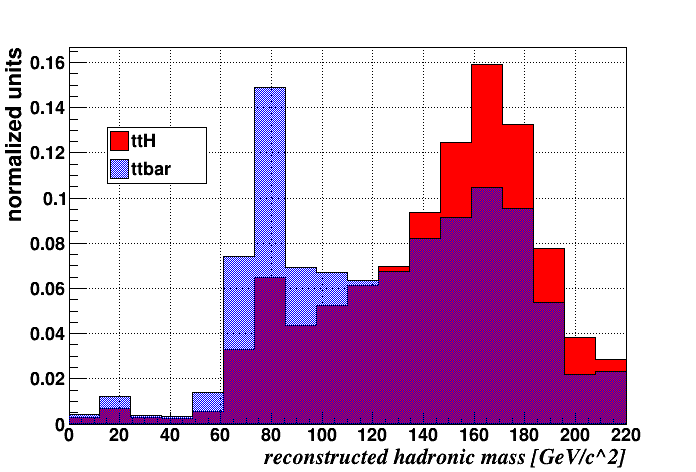
\includegraphics[width=0.4\textwidth]{plots_reconstruction/had_top_mass.png}
   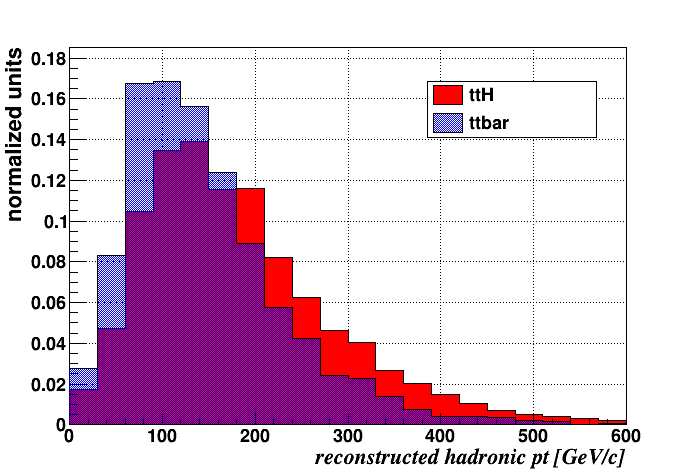
\includegraphics[width=0.4\textwidth]{plots_reconstruction/had_top_pt.png}\\
   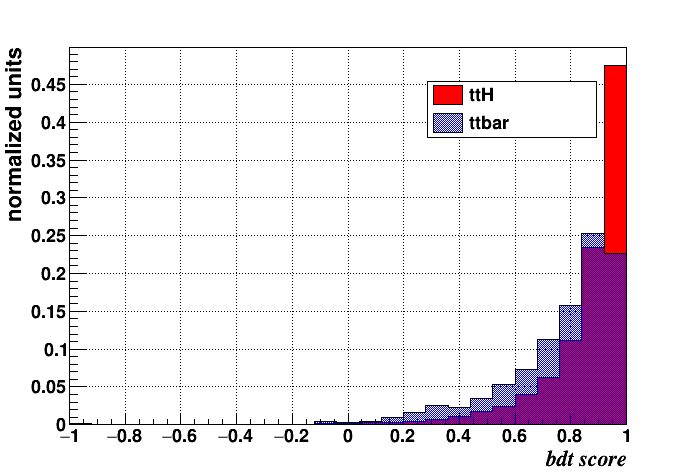
\includegraphics[width=0.4\textwidth]{plots_reconstruction/bdt_score.png}
   \caption{Output variables used for discrimination against semi-leptonic $t\bar{t}$.}
  \label{reconstruction:outputVars}
\end{figure}

\begin{figure}[htb]
 \centering
   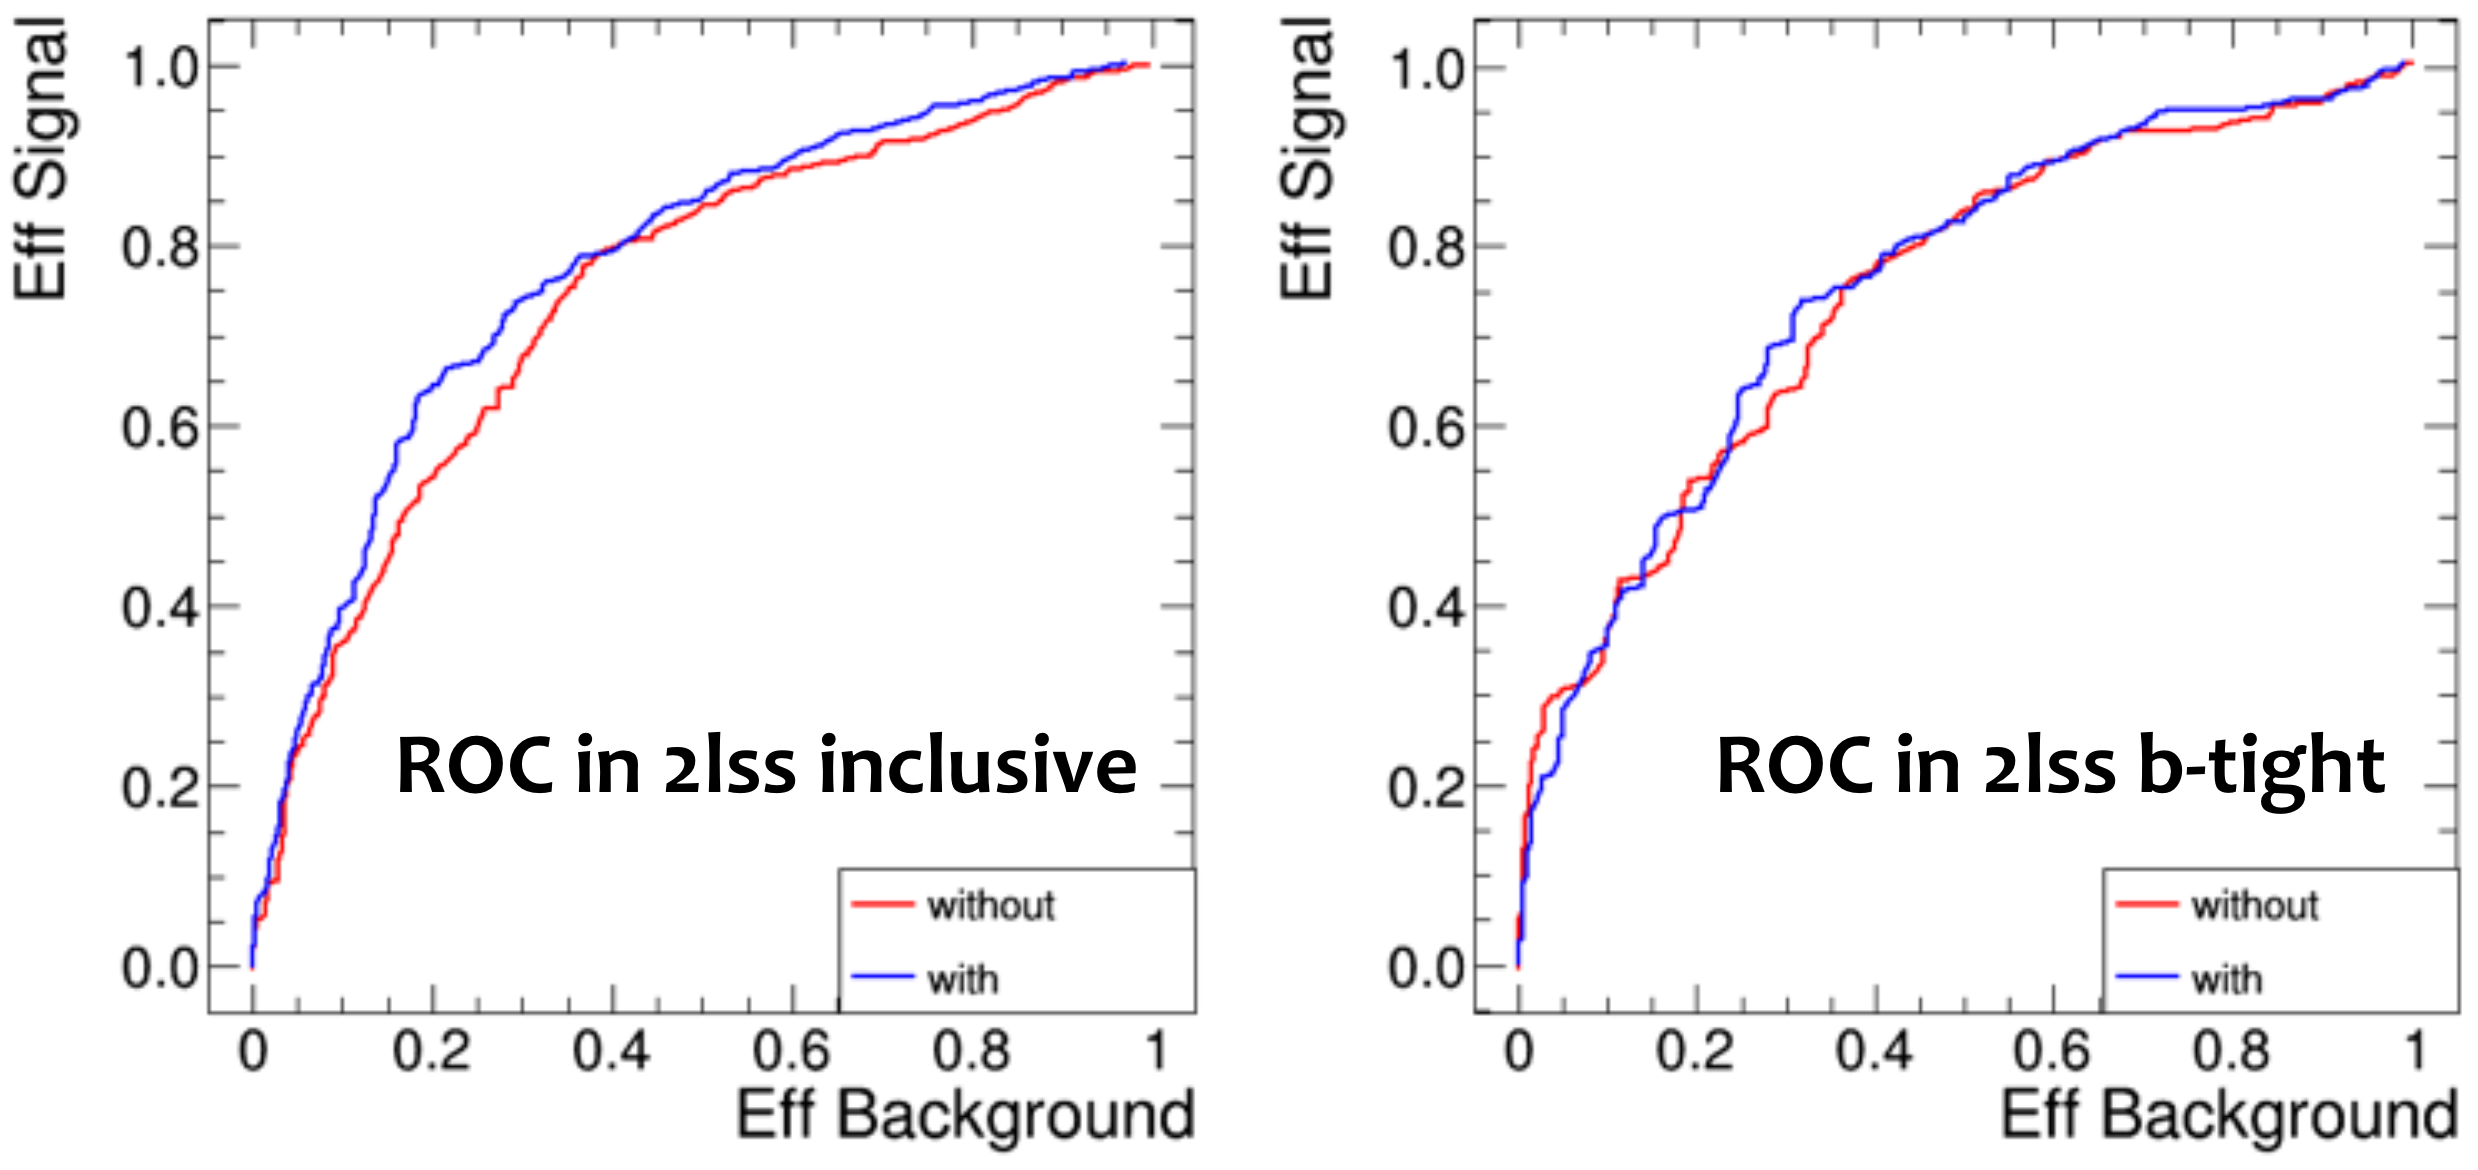
\includegraphics[width=0.7\textwidth]{plots_reconstruction/roc_improvement.png}
   \caption{ROC curve of signal extraction BDT with and without reconstruction variables evaluated against $t\bar{t}$.}
  \label{reconstruction:roc}
\end{figure}


\begin{figure}[htb]
 \centering
   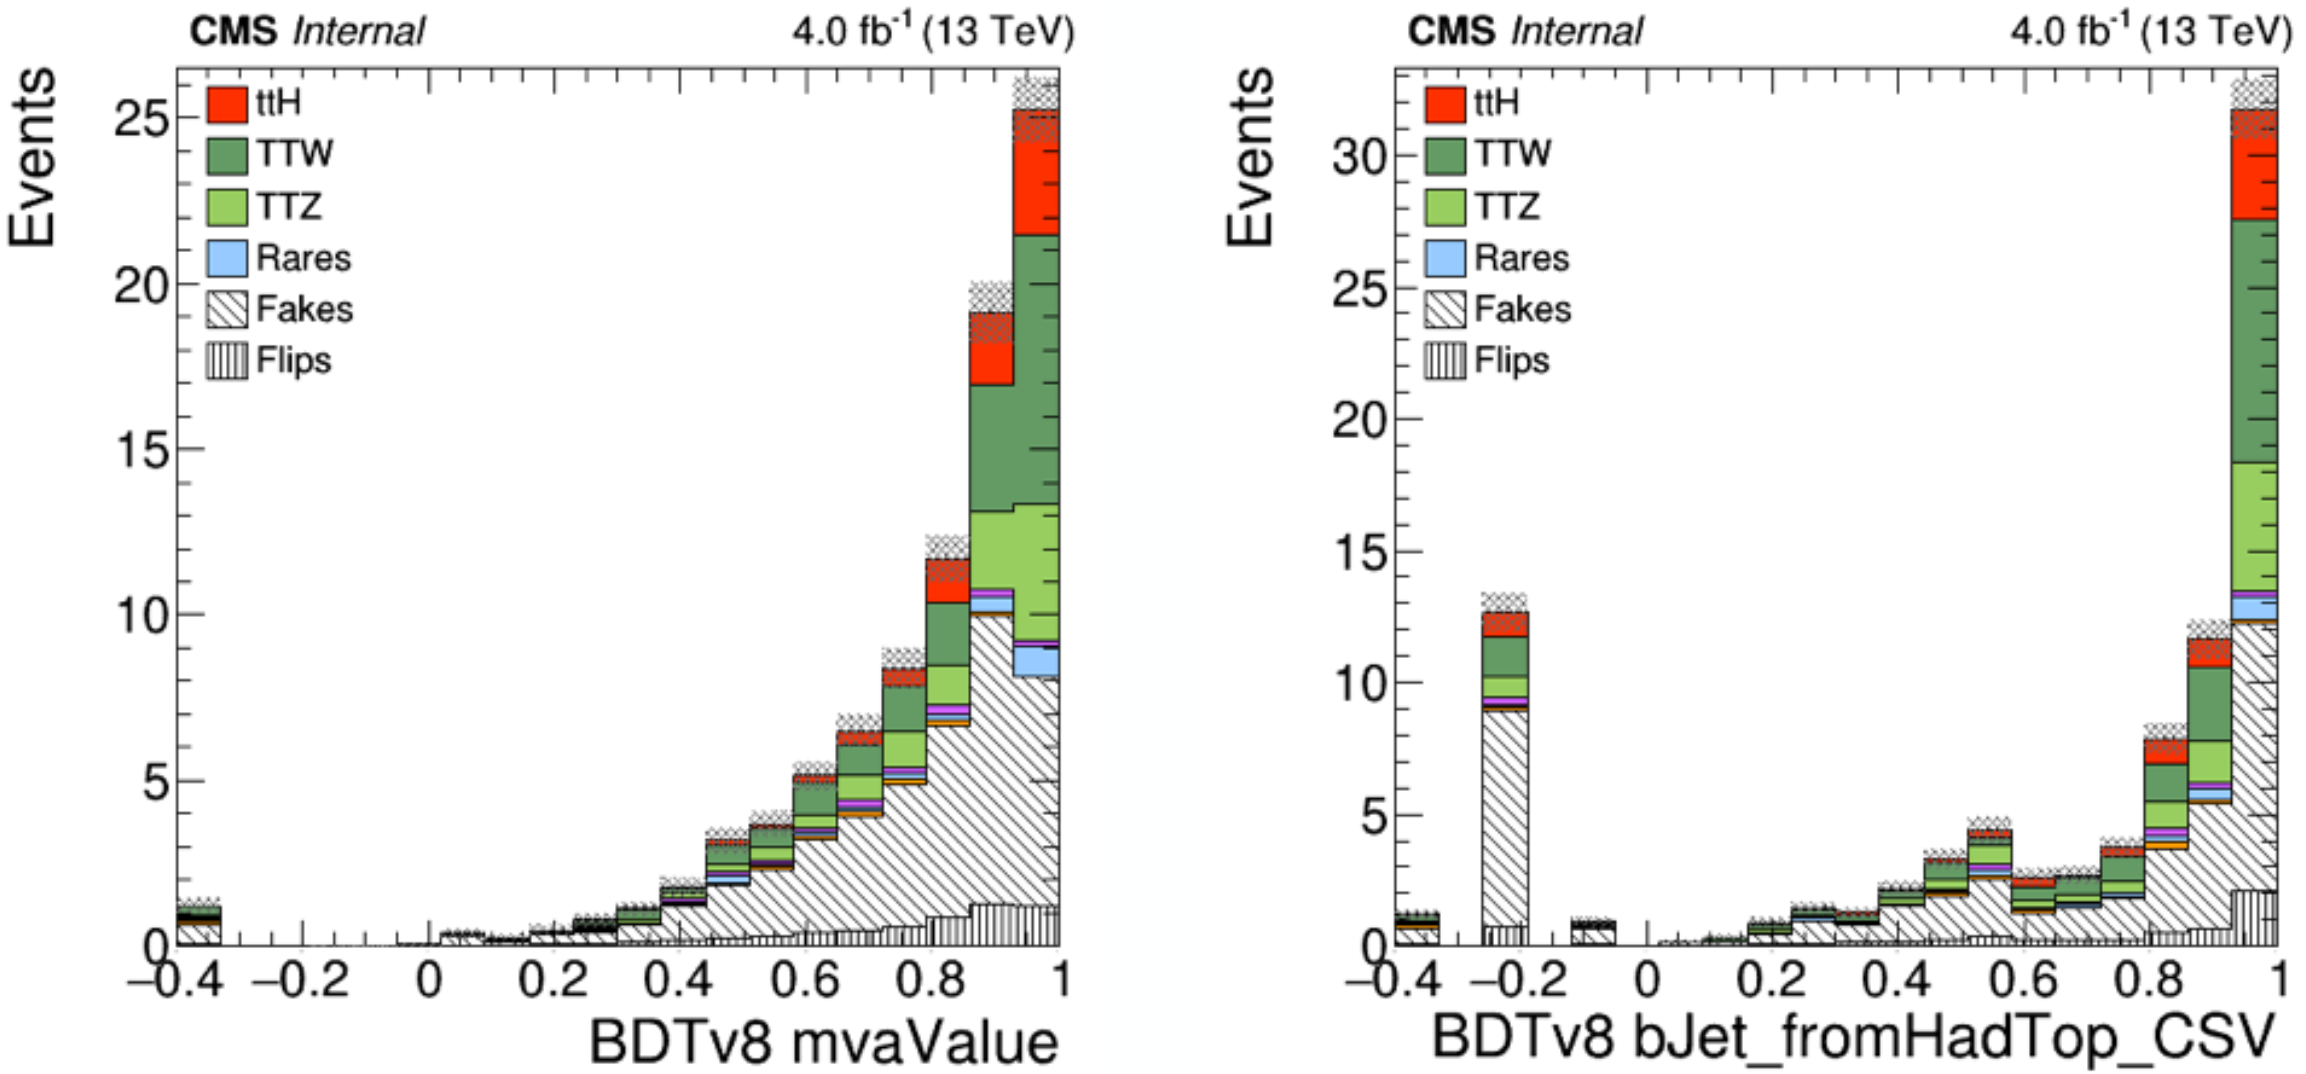
\includegraphics[width=0.7\textwidth]{plots_reconstruction/reconstruction_mva_csv_signal_region.png}
   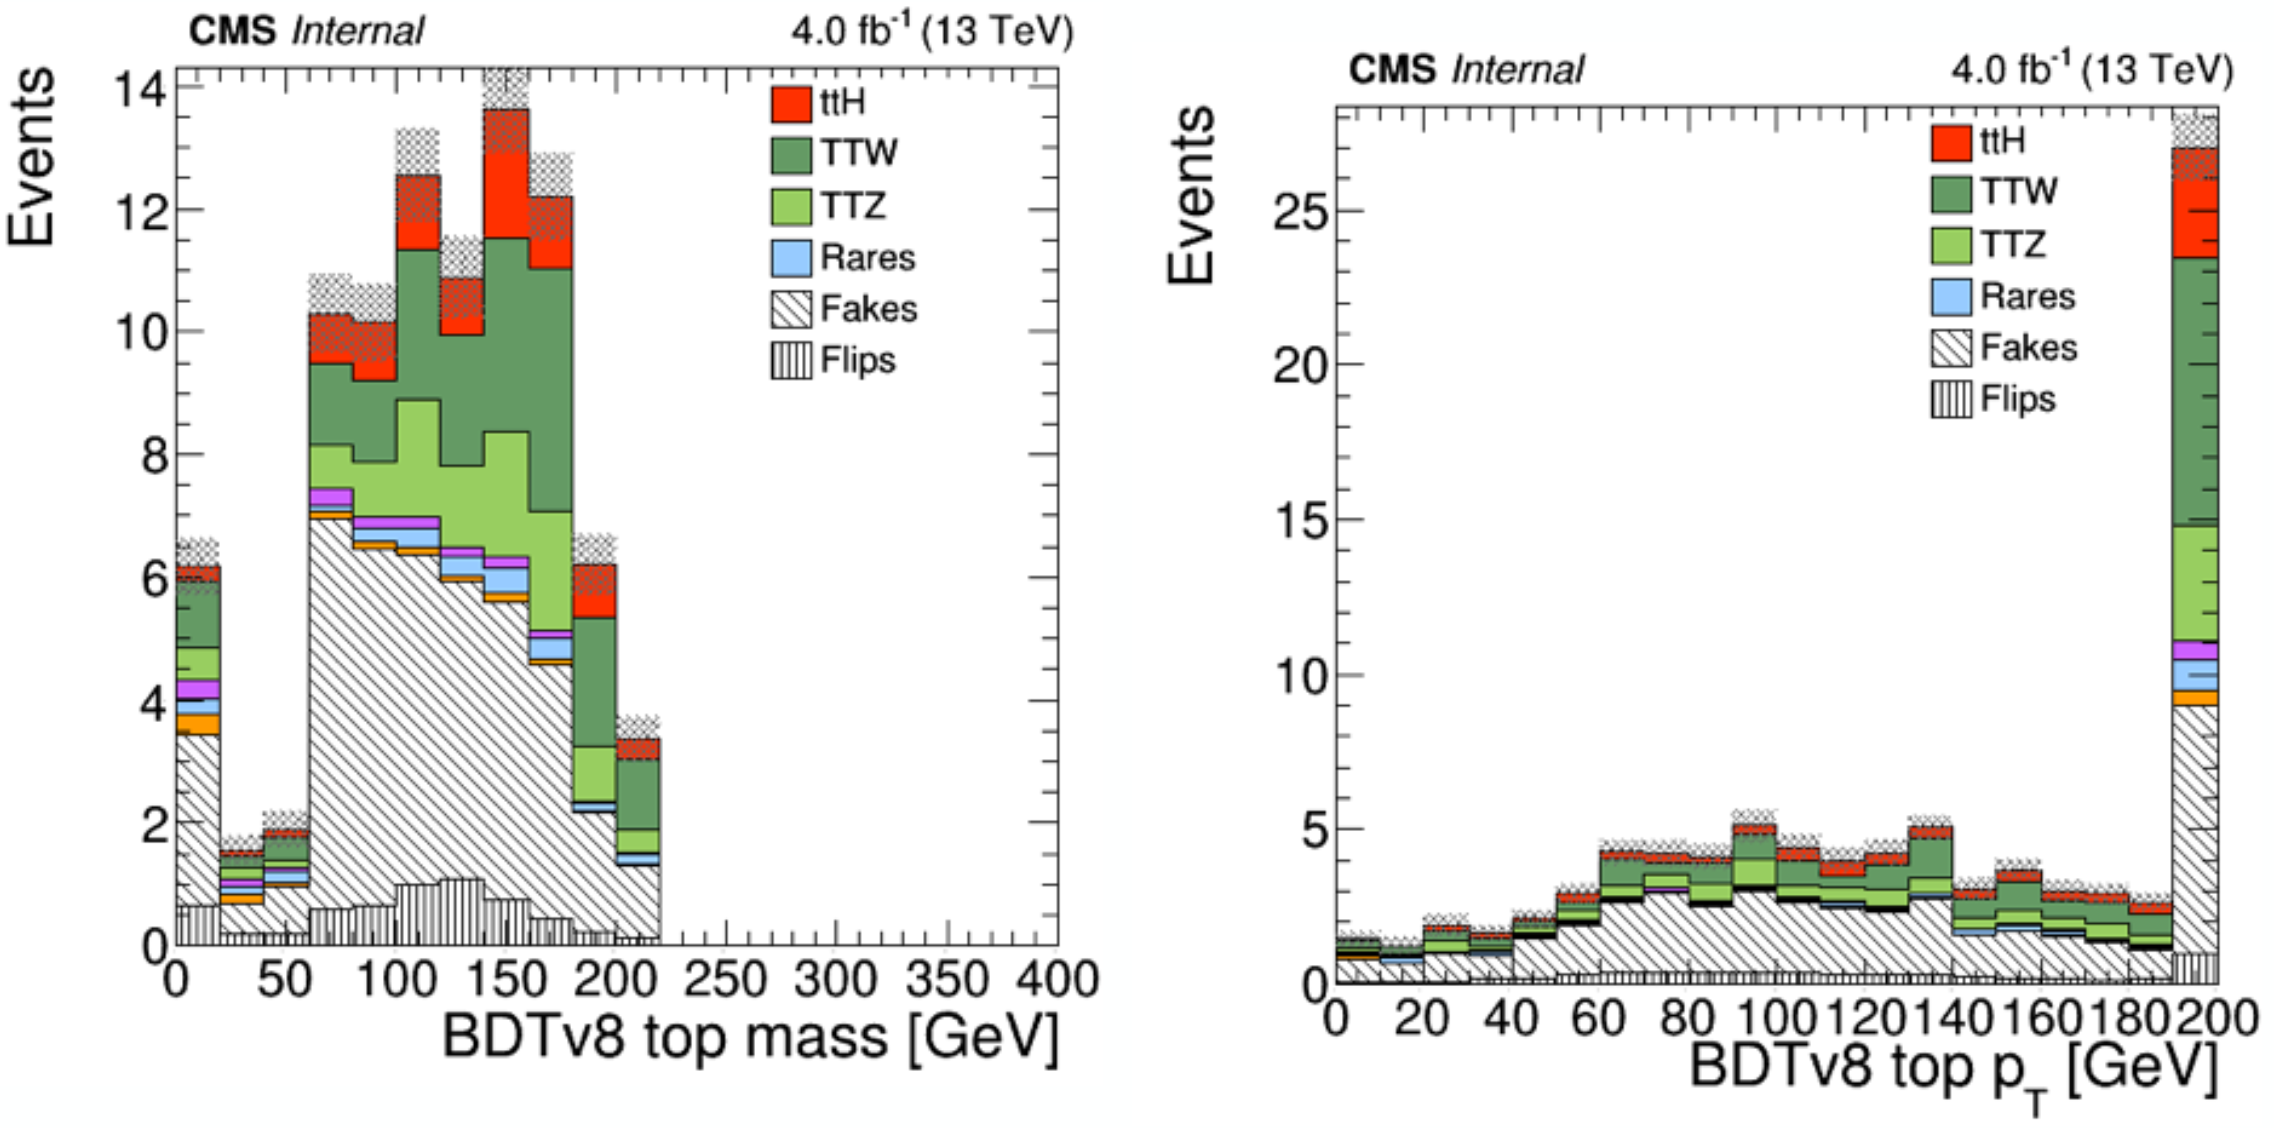
\includegraphics[width=0.7\textwidth]{plots_reconstruction/reconstruction_topmass_toppt_signal_region.png}
   \caption{Event reconstruction variables in the 2lss signal region.}
  \label{reconstruction:vars_signal_region}
\end{figure}

\begin{figure}[htb]
 \centering
   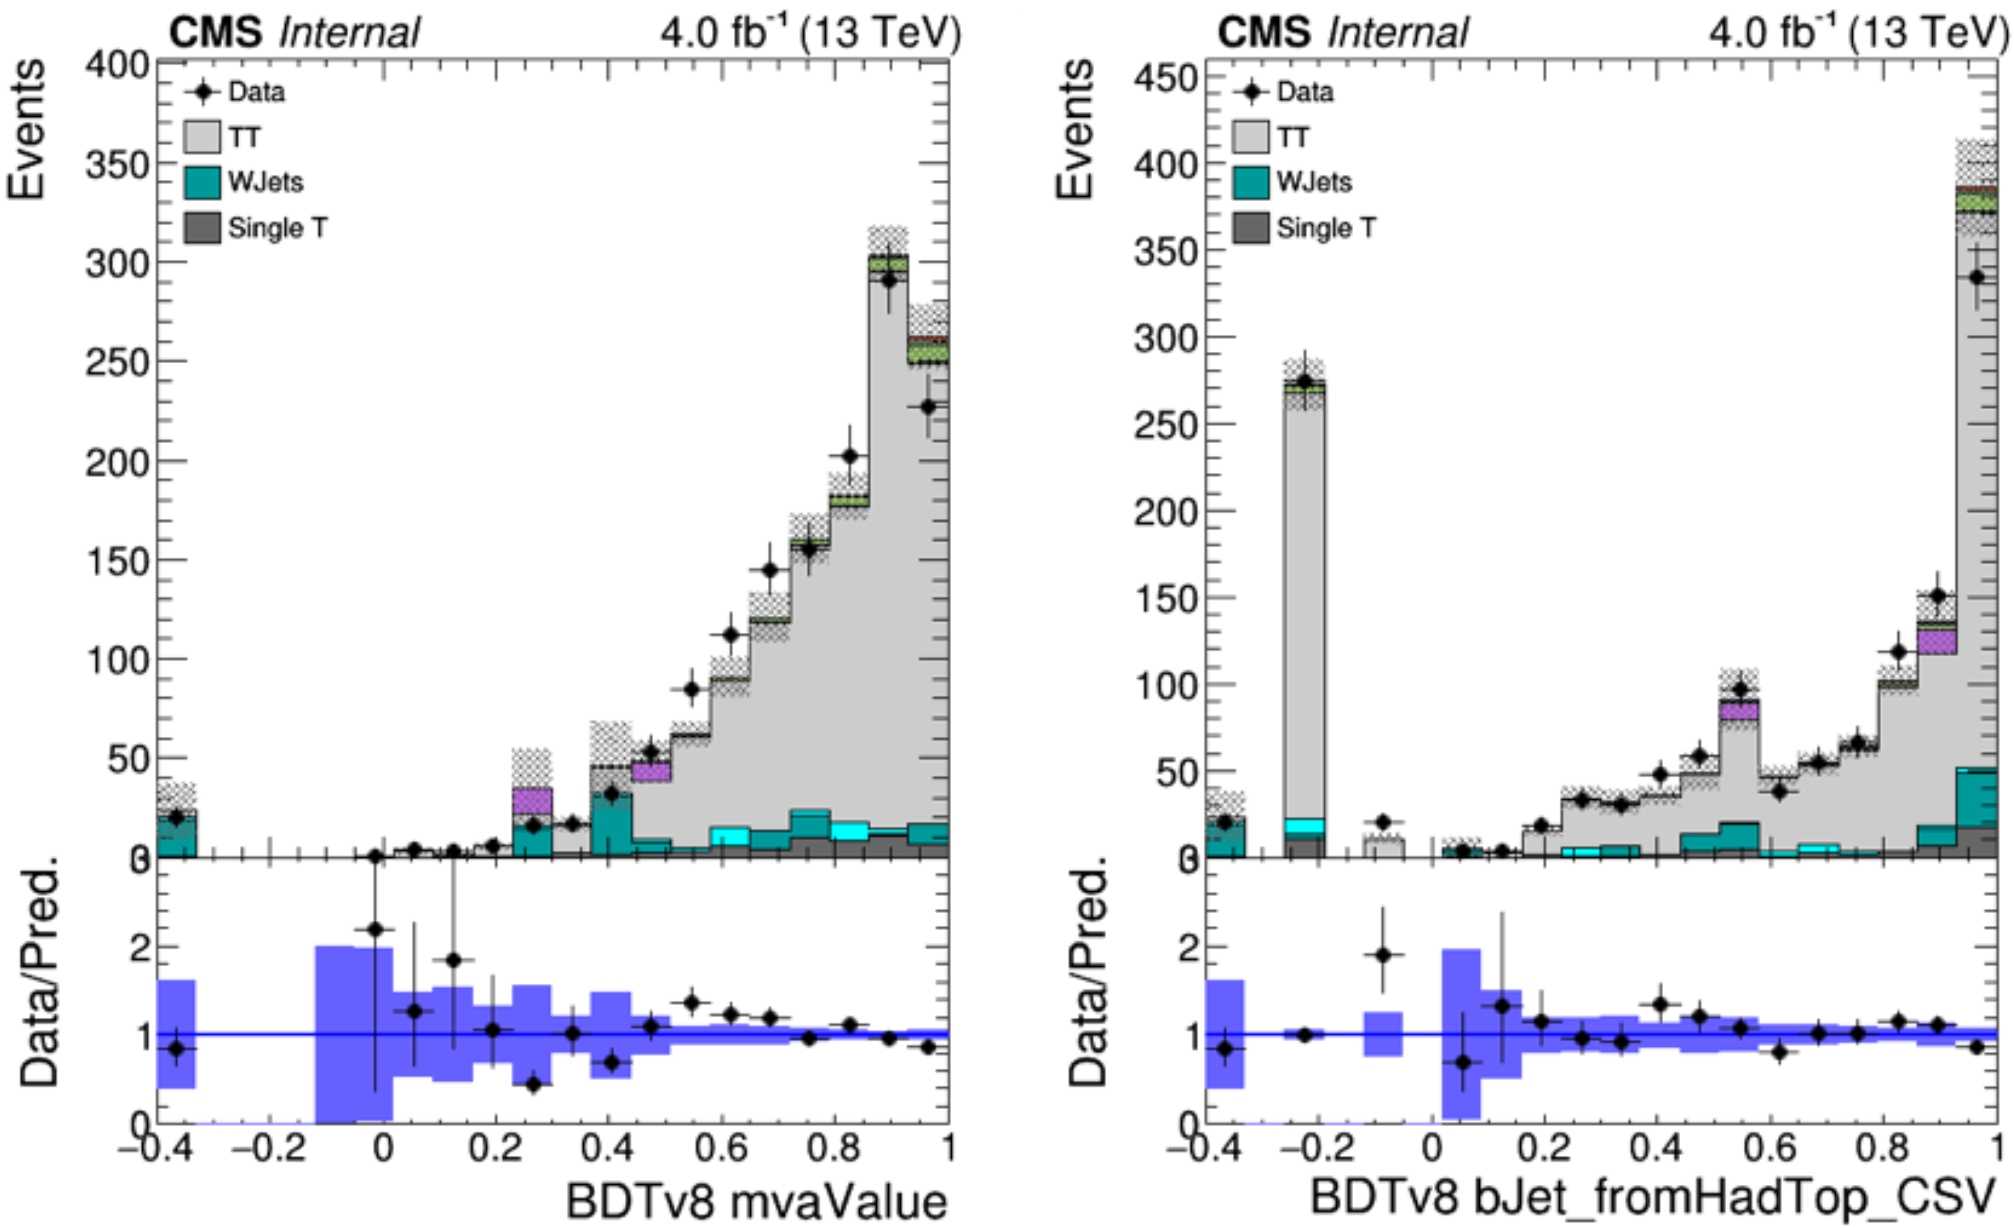
\includegraphics[width=0.7\textwidth]{plots_reconstruction/reconstruction_mva_csv_application_region.png}
   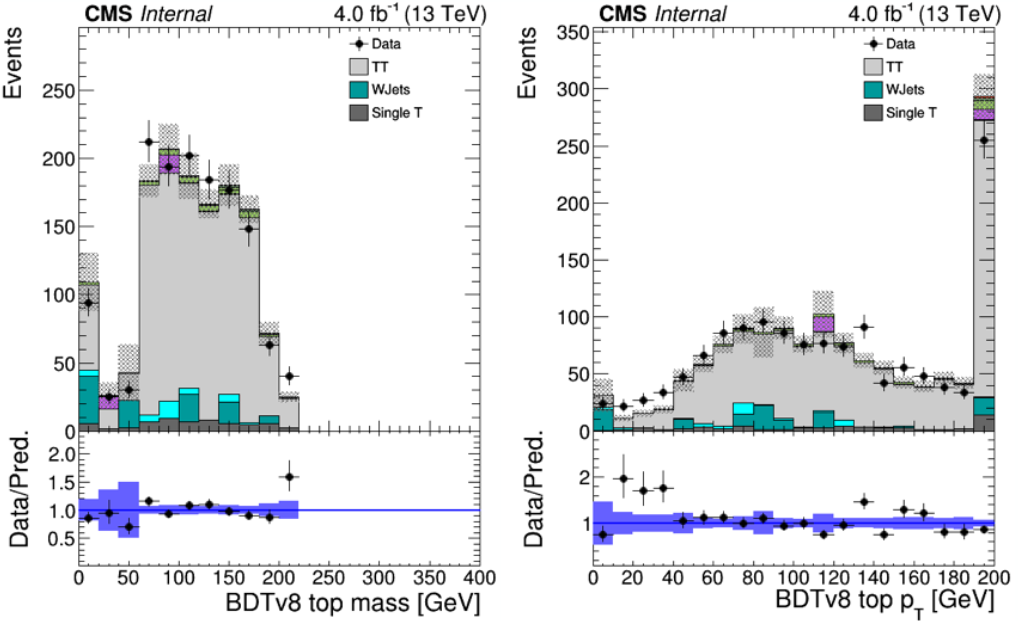
\includegraphics[width=0.7\textwidth]{plots_reconstruction/reconstruction_topmass_toppt_application_region.png}
   \caption{Event reconstruction variables in the 2lss application region.}
  \label{reconstruction:vars_application_region}
\end{figure}

\begin{figure}[htb]
 \centering
   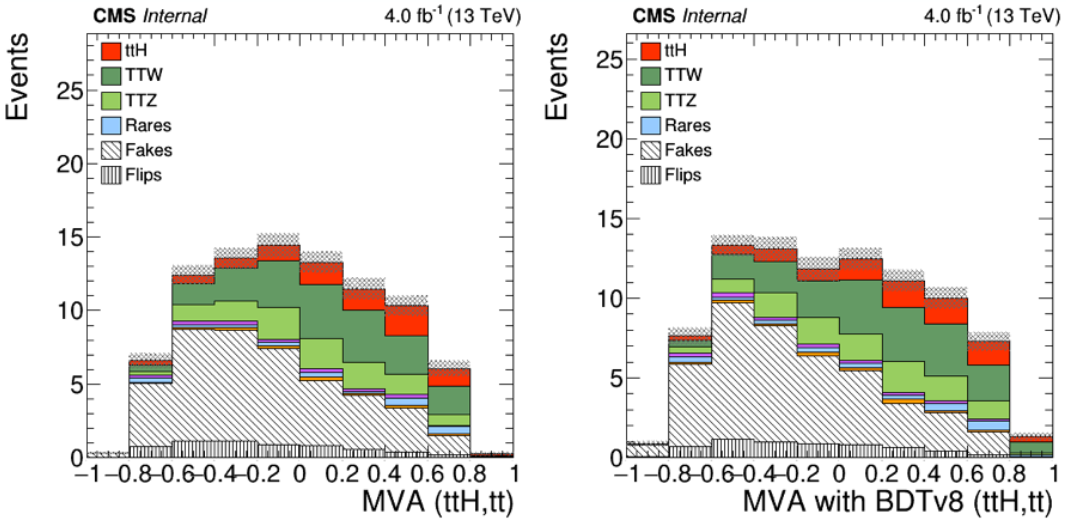
\includegraphics[width=0.7\textwidth]{plots_reconstruction/reconstruction_extraction_mva_output.png}
   \caption{Signal extraction MVA output with and with out signal extraction.}
  \label{reconstruction:extraction_output}
\end{figure}
